% =====================================================================
% Guía del estudiante -- Geometría 5° -- Trimestre I
% Hilo conductor: Cali, mi ciudad (Tatiana, la visitante del ejemplo del DBA 7)
% Plan: guia-periodo-I-ubicacion.plan.md (etapas A, B y C, 2026-09-14)
% Temas (curriculo/programacion.csv, sesiones 002-008):
%   referencia, plano, trayectorias, mapas
% Ejercicios: recursos/banco/matematicas/ubicacion-5.py y plano-cartesiano-5.py
% =====================================================================
\documentclass[11pt]{article}
\makeatletter\def\input@path{{../../../../plantillas/estilo/}}\makeatother
\usepackage{mmcantillo}

% ======================== DATOS DE LA GUÍA ============================
\tipodocumento{Guía del estudiante}
\asignatura{Geometría}
\titulo{Ubicarse, orientarse y llegar}
\grado{5°}
\periodo{I}
\hiloconductor{Cali, mi ciudad}
% ======================================================================
% DBA: matematicas grado 5 · DBA 7 — Resuelve y propone situaciones en las que es necesario
% describir y localizar la posición y la trayectoria de un objeto con referencia al plano
% cartesiano. (dba/matematicas/grados/grado05.tex)

% Cuadrícula de coordenadas del primer cuadrante: \ejes{xmax}{ymax}
\newcommand{\ejes}[2]{%
  \draw[gray!45] (0,0) grid (#1,#2);
  \draw[->, thick] (0,0) -- (#1+0.5,0) node[right, font=\small] {$x$};
  \draw[->, thick] (0,0) -- (0,#2+0.5) node[above, font=\small] {$y$};
  \foreach \i in {1,...,#1}
    \node[below, font=\scriptsize, text height=1.5ex, text depth=0.25ex] at (\i,0) {\i};
  \foreach \j in {1,...,#2} \node[left, font=\scriptsize] at (0,\j) {\j};
  \node[below left, font=\scriptsize] at (0,0) {0};}
% Rosa de los vientos pequeña en (#1)
\newcommand{\rosa}[1]{%
  \begin{scope}[shift={(#1)}, font=\scriptsize]
    \draw[->] (0,0) -- (0,0.6) node[above] {N};
    \draw (0,0) -- (0,-0.6) node[below] {S};
    \draw (0,0) -- (0.6,0) node[right] {E};
    \draw (0,0) -- (-0.6,0) node[left] {O};
  \end{scope}}

\begin{document}

\encabezado

% ---------------------------------------------------------------------
% 1. Frase introductoria
% ---------------------------------------------------------------------
% verificado: https://it.wikisource.org/wiki/Il_Saggiatore_(Favaro)/6 — «La filosofia è scritta in questo grandissimo libro che continuamente ci sta aperto innanzi a gli occhi (io dico l'universo)… Egli è scritto in lingua matematica, e i caratteri son triangoli, cerchi, ed altre figure geometriche»
\frase{La filosofía está escrita en ese grandísimo libro que continuamente está abierto ante
nuestros ojos (digo, el universo)\ldots\ Está escrito en lengua matemática, y sus caracteres
son triángulos, círculos y otras figuras geométricas.}
{Galileo Galilei, \emph{Il Saggiatore} (1623), trad. propia}

% ---------------------------------------------------------------------
% 2. Introducción
% ---------------------------------------------------------------------
\seccion{Introducción}

Con esa frase, Galileo~\cite{galileo1623} quería decir que, para entender el mundo, hace falta
el idioma de la geometría. Este trimestre lo vamos a comprobar con algo muy práctico:
\textbf{no perderse}. Decir dónde está un puesto del salón, explicar cómo llegar a un parque o
encontrar un lugar en un mapa son problemas de geometría, y se resuelven con dos números y un
acuerdo.

Nuestro hilo conductor es \textbf{Cali, mi ciudad}. Tatiana es una visitante que acaba de
llegar a Cali y no conoce nada: ni el colegio, ni el barrio, ni las calles. En cada tema le
daremos una herramienta nueva para ubicarse, y al final le escribiremos un mensaje con un
recorrido completo por el barrio, tan claro que pueda seguirlo sola.

\textbf{Al terminar este trimestre podrás:}
\begin{itemize}
  \item describir la posición de un objeto con un sistema de referencia: filas y columnas, o
        puntos cardinales;
  \item reconocer los elementos del plano cartesiano (ejes, origen, cuadrantes, coordenadas) y
        ubicar y leer puntos con pares ordenados;
  \item describir, dibujar y comparar trayectorias en una cuadrícula;
  \item localizar lugares en un mapa a partir de sus coordenadas y escribir un recorrido para
        otra persona.
\end{itemize}

Este trimestre trabaja el siguiente Derecho Básico de Aprendizaje del Ministerio de Educación
Nacional~\cite{mendba}:

\begin{dba}[Grado 5 · DBA 7]
Resuelve y propone situaciones en las que es necesario describir y localizar la posición y la
trayectoria de un objeto con referencia al plano cartesiano.
\end{dba}

% ---------------------------------------------------------------------
% 3. Marco teórico
% ---------------------------------------------------------------------
\seccion{Marco teórico}

\subsubsection*{¿Dónde queda?}

«Al lado de la ventana», «detrás de la iglesia», «dos cuadras después del parque»: así
describimos casi siempre dónde está algo. Estas descripciones sirven entre personas que conocen
el lugar, pero no le sirven a quien llega por primera vez, como Tatiana. Para ella hace falta un
\textbf{sistema de referencia}: un punto de partida y unas reglas que todos entiendan igual.

\subsubsection*{Los puntos cardinales}

El sistema más antiguo usa el Sol. Por el \textbf{oriente} (o este) sale y por el
\textbf{occidente} (u oeste) se oculta. Si te paras mirando hacia el oriente, el
\textbf{norte} queda a tu izquierda y el \textbf{sur} a tu derecha. Por costumbre, los mapas se
dibujan con el norte hacia arriba; por eso, en un mapa, el oriente queda a la derecha y el
occidente a la izquierda. En Colombia, el Instituto Geográfico Agustín Codazzi elabora la
cartografía oficial del país y publica sus mapas, en los que cada lugar tiene
coordenadas~\cite{igac}.

\subsubsection*{Descartes: ponerle números al espacio}

En 1637, el filósofo y matemático francés René Descartes publicó \emph{La geometría}, como un
apéndice de su \emph{Discurso del método}~\cite{descartes1637}. Allí mostró cómo describir la
posición de un punto con \textbf{dos números}: dos distancias medidas a partir de dos rectas de
referencia. Descartes no exigía que esas rectas fueran perpendiculares~\cite{sepdescartes}; hoy,
por comodidad, siempre las dibujamos formando un ángulo recto. En su honor, el sistema se llama
\textbf{plano cartesiano}.

Se cuenta que Descartes tuvo la idea acostado en su cama, mirando una mosca que caminaba por el
techo: ¿cómo decir con números dónde estaba la mosca?~\cite{nrichmosca}. Es solo una leyenda,
pero explica muy bien el problema que resolvió.

\subsubsection*{Katherine Johnson: trayectorias que llegaron al espacio}

Más de trescientos años después, en Estados Unidos, la matemática \textbf{Katherine Johnson}
calculó en la NASA la trayectoria del primer vuelo espacial tripulado de su país, el de Alan
Shepard, en 1961. En 1962, antes de que John Glenn diera la vuelta a la Tierra, las cuentas las
hizo un computador, y Glenn pidió que ella repitiera a mano los mismos cálculos. Según la NASA,
dijo:

% verificado: https://www.nasa.gov/centers-and-facilities/langley/katherine-johnson-biography/ — Glenn: «If she says they're good, then I'm ready to go» (trad. propia)
\begin{cita}{John Glenn, citado por la NASA~\cite{nasajohnson} (trad. propia)}
Si ella dice que están bien, entonces estoy listo para salir.
\end{cita}

Es decir: Glenn confiaba más en las cuentas cuidadosas de una persona que en una máquina nueva.
Una trayectoria es justo lo que vamos a dibujar en esta guía: una sucesión de posiciones, una
detrás de otra.

% ---------------------------------------------------------------------
% 4. Temas
% ---------------------------------------------------------------------
\tema{Sistemas de referencia}\label{tema:referencia}

\begin{hilo}
Tatiana llega al colegio y pregunta dónde se sienta Andrés, un estudiante de 5°. Alguien le
responde: «al lado de la cafetería, detrás de Sofía». Pero Tatiana no sabe dónde está la
cafetería ni quién es Sofía. Necesita algo que no dependa de lo que ya conoce: un sistema.
\end{hilo}

\begin{definicion}[Sistema de referencia]
Un \textbf{sistema de referencia} es un acuerdo para decir dónde está algo sin depender de
quién lo mire: un punto de partida y unas reglas que todos usan igual.
\end{definicion}

En el salón usamos este acuerdo: las \textbf{filas} se nombran con letras, de la $A$ a la $D$,
empezando por la más cercana al tablero, y las \textbf{columnas} con números, del 1 al 5, de
izquierda a derecha mirando al tablero. La posición se escribe como un par
\textbf{(fila, columna)}: $(B, 4)$ se lee «fila $B$, columna 4».

\begin{center}
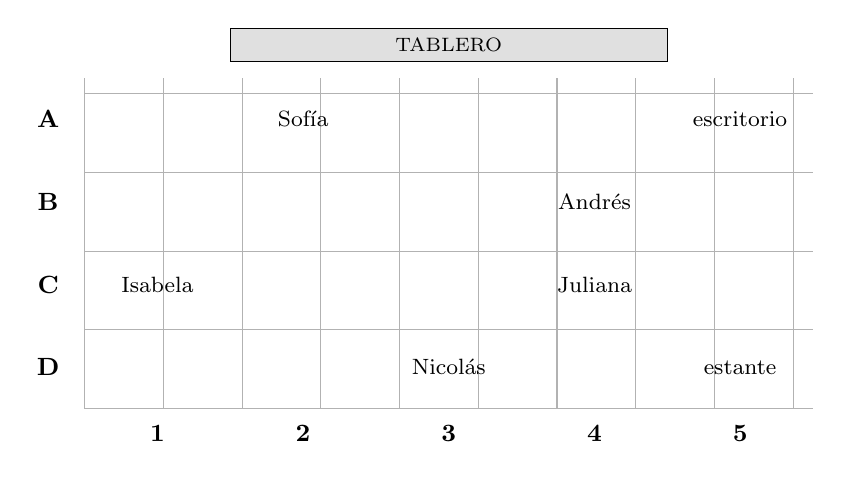
\begin{tikzpicture}[x=1.85cm, y=1.05cm, font=\footnotesize]
  \draw[gray!60] (0,0) grid (5,4);
  \foreach \x/\n in {0.5/1, 1.5/2, 2.5/3, 3.5/4, 4.5/5}
    \node[font=\small\bfseries] at (\x,-0.3) {\n};
  \foreach \y/\l in {3.5/A, 2.5/B, 1.5/C, 0.5/D}
    \node[font=\small\bfseries] at (-0.25,\y) {\l};
  \draw[fill=black!12] (1,4.2) rectangle (4,4.6);
  \node[font=\scriptsize] at (2.5,4.4) {TABLERO};
  \node at (1.5,3.5) {Sofía};
  \node at (4.5,3.5) {escritorio};
  \node at (3.5,2.5) {Andrés};
  \node at (0.5,1.5) {Isabela};
  \node at (3.5,1.5) {Juliana};
  \node at (2.5,0.5) {Nicolás};
  \node at (4.5,0.5) {estante};
\end{tikzpicture}

{\footnotesize Cuadrícula del salón de 5°: filas desde el tablero, columnas de izquierda a derecha.}
\end{center}

% Ejercicio: ubicacion-5-001
\begin{ejemplo}[Leer la cuadrícula]
Andrés está en $(B, 4)$: fila $B$, columna 4. Y si Tatiana busca el puesto $(D, 3)$, cuenta
cuatro filas desde el tablero y tres columnas desde la izquierda: allí está Nicolás. Nunca ha
entrado al salón, y aun así lo encuentra.
\end{ejemplo}

\textbf{El orden importa.} El par dice primero la fila y después la columna. Y también importa
desde dónde se cuenta: si alguien contara las filas desde el fondo del salón, el mismo par
señalaría otro puesto. Por eso un sistema de referencia es, ante todo, un \emph{acuerdo}.

\textbf{Los puntos cardinales en un plano.} En el plano del colegio, el norte está arriba, como
en los mapas. Desde el patio, cada lugar queda en una dirección:

\begin{center}
\begin{minipage}{\linewidth}
\centering
\begin{tikzpicture}[font=\footnotesize, lugar/.style={draw, minimum width=2.1cm, minimum height=0.75cm}]
  \node[draw, dashed, minimum width=2.1cm, minimum height=0.75cm] (p) at (0,0) {patio};
  \node[lugar] at (0,1.3) {biblioteca};
  \node[lugar] at (2.8,0) {cafetería};
  \node[lugar] at (0,-1.3) {coliseo};
  \node[lugar] at (-2.8,0) {portería};
  \rosa{5.6,0}
\end{tikzpicture}

{\footnotesize Plano del colegio (simplificado), con el norte hacia arriba.}
\end{minipage}
\end{center}

\begin{aplicacion}[Las sillas de un teatro o de un estadio]
Las boletas de un teatro o de un estadio traen la fila y el número de la silla. Miles de
personas que nunca se han visto encuentran cada una su puesto sin preguntar, porque todas usan
el mismo acuerdo: desde dónde se cuentan las filas y en qué sentido se numeran las sillas.
\end{aplicacion}

\begin{preguntas}
% Ejercicio: ubicacion-5-002
\pregunta Usa la cuadrícula del salón. Escribe la posición (fila, columna) de Sofía y de
Isabela, y di qué hay en $(A, 5)$ y en $(D, 5)$.
\renglones{2}
% Ejercicio: ubicacion-5-003
\pregunta Camilo le dice a Tatiana que Andrés está en $(C, 4)$, porque contó las filas desde el
fondo del salón y no desde el tablero. Encuentra el error: ¿a quién encontraría Tatiana en
$(C, 4)$? ¿Cuál es la posición correcta de Andrés y por qué?
\renglones{3}
% Ejercicio: ubicacion-5-004
\pregunta Observa el plano del colegio (el norte está arriba). Tatiana está en el patio.
\begin{opciones}
  \item ¿Qué lugar queda al norte del patio?
  \item Si camina hacia el occidente, ¿a dónde llega?
  \item Si se para mirando hacia donde sale el Sol, ¿qué lugar tiene a su izquierda y cuál a su
        espalda?
\end{opciones}
\renglones{3}
% Ejercicio: ubicacion-5-005 — manual-pendiente: entra cuando la docente apruebe la respuesta
% modelo (python3 tools/ejercicios.py aprobar ubicacion-5-005).
% \pregunta Diseña un sistema de referencia para la biblioteca del colegio o para el
% parqueadero: dibuja la cuadrícula, nombra filas y columnas y escribe en dos o tres renglones
% las reglas, para que Tatiana pueda encontrar tres lugares que tú marques.
% \espacio{4cm}
\end{preguntas}

\begin{resumen}
\begin{itemize}
  \item Un sistema de referencia es un acuerdo: un punto de partida y unas reglas comunes.
  \item En el salón, la posición es el par (fila, columna), contando las filas desde el tablero.
  \item Si cambia el orden o el punto de partida, el mismo par señala otro lugar.
  \item Los puntos cardinales son norte, sur, oriente y occidente; el Sol sale por el oriente, y
        en los mapas el norte va arriba.
\end{itemize}
\end{resumen}

\tema{El plano cartesiano}\label{tema:plano}

\begin{hilo}
Las letras de las filas sirven en un salón, pero se acaban pronto y no permiten medir. Para
ubicar a Tatiana en toda una ciudad hace falta algo mejor: Descartes cambió las letras por
números, y así cualquier persona, en cualquier idioma, entiende una posición.
\end{hilo}

\begin{definicion}[Plano cartesiano]
El \textbf{plano cartesiano} está formado por dos rectas numeradas perpendiculares, los
\textbf{ejes}: el horizontal es el \textbf{eje $x$} y el vertical, el \textbf{eje $y$}. Se
cortan en el \textbf{origen}, que es el punto $(0, 0)$. Cada punto se nombra con un
\textbf{par ordenado} $(x, y)$: primero cuántas unidades hacia la derecha y después cuántas
hacia arriba. Esos dos números son sus \textbf{coordenadas}.
\end{definicion}

\textbf{Un acuerdo nuevo.} En el salón decíamos primero la fila, que es un dato vertical. En el
plano cartesiano se dice primero el dato \emph{horizontal} ($x$) y después el vertical ($y$).
Es la regla que usa todo el mundo en matemáticas, y es la misma del ajedrez: la casilla «e4» es
la columna $e$ y la fila 4, primero la columna y luego la fila~\cite{fide}.

\begin{center}
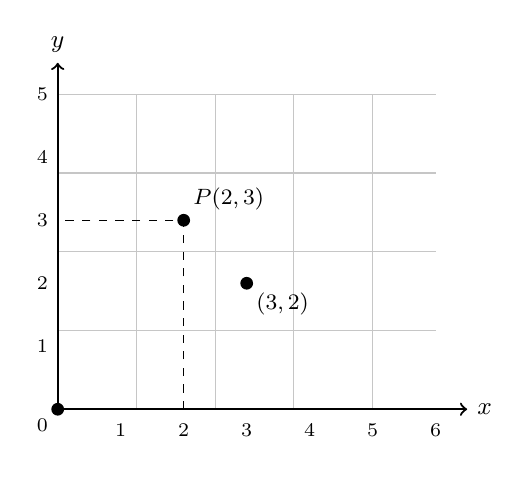
\begin{tikzpicture}[x=0.8cm, y=0.8cm]
  \ejes{6}{5}
  \draw[dashed] (2,0) -- (2,3) -- (0,3);
  \fill (2,3) circle (2.3pt) node[above right, font=\footnotesize] {$P(2, 3)$};
  \fill (3,2) circle (2.3pt) node[below right, font=\footnotesize] {$(3, 2)$};
  \fill (0,0) circle (2.3pt);
\end{tikzpicture}
\hspace{1cm}
\begin{tikzpicture}[x=0.8cm, y=0.8cm, font=\footnotesize]
  \fill[pattern=north east lines, pattern color=gray] (0,0) rectangle (2.4,2.4);
  \draw[->, thick] (-2.6,0) -- (2.7,0) node[right] {$x$};
  \draw[->, thick] (0,-2.6) -- (0,2.7) node[above] {$y$};
  \node[fill=white, inner sep=1pt] at (1.2,1.2) {I};
  \node at (-1.2,1.2) {II};
  \node at (-1.2,-1.2) {III};
  \node at (1.2,-1.2) {IV};
  \node[below left] at (0,0) {$O$};
\end{tikzpicture}

{\footnotesize Izquierda: el punto $P(2, 3)$ y el punto $(3, 2)$. Derecha: los cuatro
cuadrantes; en 5° trabajamos en el primero (rayado).}
\end{center}

% Ejercicio: ubicacion-5-006
\begin{ejemplo}[Ubicar el punto $P(2, 3)$]
Desde el origen se avanzan 2 unidades hacia la derecha y luego 3 hacia arriba: las líneas
punteadas muestran el camino. Si se hace al revés, 3 a la derecha y 2 hacia arriba, se llega al
punto $(3, 2)$, que es otro lugar. Por eso el par se llama \emph{ordenado}.
\end{ejemplo}

\textbf{Los cuadrantes.} Los dos ejes dividen el plano en cuatro regiones, los
\textbf{cuadrantes}, que se numeran I, II, III y IV. En el primero, las dos coordenadas son
positivas. Los otros tres necesitan números negativos, que estudiarás en grados posteriores;
este trimestre trabajamos solo en el primer cuadrante y sobre los ejes.

\textbf{Puntos cardinales en el plano.} Si el norte está arriba, avanzar hacia el
\textbf{oriente} es moverse a la derecha (crece $x$) y avanzar hacia el \textbf{norte} es
subir (crece $y$).

% Ejercicio: ubicacion-5-007
\begin{ejemplo}[El banco del barrio]
El hotel de Tatiana está en el origen. El banco queda 3 cuadras al oriente y 2 al norte: su par
ordenado es $(3, 2)$, porque el oriente da el primer número y el norte, el segundo.
\end{ejemplo}

\begin{aplicacion}[La batalla naval y las pantallas]
En el juego de la batalla naval, cada disparo se anuncia con dos datos, y el otro jugador sabe
exactamente a qué casilla apuntaste. La pantalla de un celular funciona igual: está hecha de
puntos de luz, y el programa ubica cada uno con dos números, cuántos hacia la derecha y cuántos
hacia arriba o hacia abajo.
\end{aplicacion}

\Needspace{14\baselineskip}
\begin{preguntas}
% Ejercicio: plano-cartesiano-5-005
\pregunta ¿Qué par ordenado representa el origen de cualquier plano cartesiano?
\renglones{1}
% Ejercicio: ubicacion-5-008
\pregunta Escribe las coordenadas de los puntos $A$, $B$, $C$, $D$ y $E$ del plano. ¿Cuáles
están sobre un eje y sobre cuál?

\begin{center}
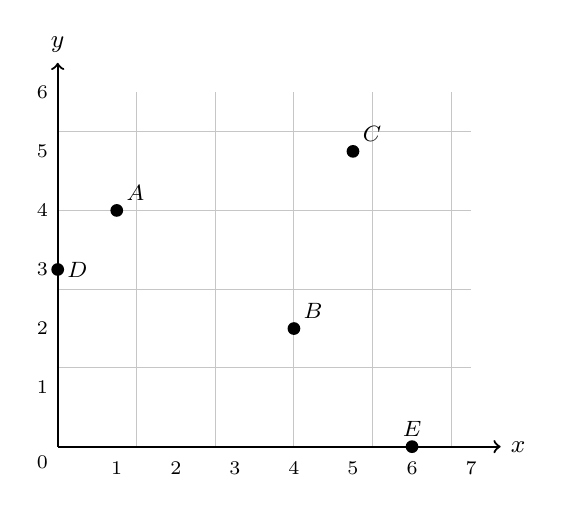
\begin{tikzpicture}[x=0.75cm, y=0.75cm, font=\footnotesize]
  \ejes{7}{6}
  \foreach \n/\px/\py/\pos in {A/1/4/above right, B/4/2/above right, C/5/5/above right,
                               D/0/3/right, E/6/0/above}
    {\fill (\px,\py) circle (2.3pt); \node[\pos] at (\px,\py) {$\n$};}
\end{tikzpicture}
\end{center}
\renglones{2}
% Ejercicio: ubicacion-5-010
\pregunta El hotel de Tatiana está en el origen. En a) y b), escribe el par ordenado del lugar;
en c) y d), escribe con puntos cardinales cómo llegar a ese punto desde el hotel.
\begin{opciones*}(2)
  \item 4 cuadras al oriente y 1 al norte.
  \item 5 cuadras al norte.
  \item $(6, 2)$.
  \item $(3, 0)$.
\end{opciones*}
\renglones{2}
% Ejercicio: ubicacion-5-009
\pregunta Ponemos la cuadrícula del salón sobre un plano cartesiano: las columnas 1 a 5 son
los valores de $x$, y las filas se numeran de abajo hacia arriba ($D$ es $y = 1$, $C$ es
$y = 2$, $B$ es $y = 3$ y $A$, la del tablero, es $y = 4$). Escribe la posición de Andrés
como (fila, columna) y como par $(x, y)$. ¿Por qué el dato de la columna pasó a ser el
primero?
\renglones{4}
% Ejercicio: ubicacion-5-011
\pregunta Tres vértices de un rectángulo son $(1, 1)$, $(5, 1)$ y $(5, 4)$. Ubícalos en papel
cuadriculado. ¿Cuál es el cuarto vértice? ¿Cuánto miden la base y la altura?
\espacio{3.5cm}
\end{preguntas}

\begin{resumen}
\begin{itemize}
  \item El plano cartesiano tiene dos ejes perpendiculares, $x$ (horizontal) e $y$
        (vertical), que se cortan en el origen $(0, 0)$.
  \item Un punto se nombra con el par ordenado $(x, y)$: primero hacia la derecha, después
        hacia arriba. $(2, 5)$ y $(5, 2)$ son puntos distintos.
  \item En el salón decíamos (fila, columna); en el plano se dice primero el dato horizontal.
  \item Los ejes forman cuatro cuadrantes; en 5° trabajamos en el primero.
  \item Con el norte arriba: oriente = hacia la derecha ($x$), norte = hacia arriba ($y$).
\end{itemize}
\end{resumen}

\tema{Trayectorias}\label{tema:trayectorias}

\begin{hilo}
Tatiana ya sabe dónde está su hotel y dónde está el zoológico. Ahora quiere saber cómo ir de uno
al otro. Katherine Johnson no calculaba un solo punto, sino el camino completo de una nave: una
sucesión de posiciones. Eso es una trayectoria.
\end{hilo}

\begin{definicion}[Trayectoria]
La \textbf{trayectoria} es el camino que sigue un objeto al moverse de un lugar a otro. En una
cuadrícula se describe de dos maneras: con \textbf{instrucciones} («3 cuadras al oriente, 2 al
norte») o con la \textbf{lista de puntos} por donde pasa y donde gira. Su \textbf{longitud} es
el total de cuadras recorridas.
\end{definicion}

En esta guía caminamos solo por las calles de la cuadrícula, es decir, por las líneas
horizontales y verticales: no se atraviesan las manzanas en diagonal.

\begin{center}
\begin{tikzpicture}[x=0.9cm, y=0.9cm, font=\footnotesize, >=Latex]
  \ejes{6}{4}
  \draw[very thick, ->] (1,1) -- (4,1) -- (4,2.9);
  \draw[very thick, dashed, ->] (1,1) -- (1,3) -- (3.9,3);
  \draw[very thick, dotted, ->] (1,0.85) -- (5.15,0.85) -- (5.15,3.15) -- (4.1,3.15);
  \fill (1,1) circle (2.5pt) node[above left, fill=white, inner sep=1pt] {hotel};
  \fill (4,3) circle (2.5pt) node[above left=3pt, fill=white, inner sep=1pt] {zoológico};
\end{tikzpicture}

{\footnotesize Tres trayectorias del hotel $(1, 1)$ al zoológico $(4, 3)$: continua, a trazos y
punteada.}
\end{center}

% Ejercicio: ubicacion-5-012
\begin{ejemplo}[Varios caminos, el mismo destino]
La trayectoria continua es «3 al oriente y 2 al norte»: gira en $(4, 1)$ y mide 5 cuadras. La de
trazos es «2 al norte y 3 al oriente»: gira en $(1, 3)$ y también mide 5 cuadras. La punteada,
«4 al oriente, 2 al norte y 1 al occidente», llega al mismo lugar pero mide 7, porque se pasa una
cuadra y tiene que devolverse. En cualquier camino más corto se recorren siempre las mismas
cuadras al oriente (3) y al norte (2); lo único que cambia es el orden.
\end{ejemplo}

\begin{aplicacion}[Las aplicaciones de mapas del celular]
Una aplicación de mapas conoce tu posición y la del destino, y calcula una trayectoria por las
calles que existen: «siga 2 cuadras, gire a la derecha». Por eso suele ofrecer varias rutas, y
si una calle está cerrada, busca otra.
\end{aplicacion}

\begin{preguntas}
% Ejercicio: ubicacion-5-013
\pregunta Tatiana sale de $(0, 2)$ y sigue estas instrucciones: 3 cuadras al oriente, 2 al
norte, 1 al oriente y 1 al sur. Dibuja la trayectoria en papel cuadriculado. ¿Por qué puntos
gira? ¿A qué punto llega? ¿Cuántas cuadras camina?
\espacio{3.5cm}
% Ejercicio: ubicacion-5-014
\Needspace{20\baselineskip}
\pregunta Observa la trayectoria dibujada: sale de $(1, 4)$, pasa por $(1, 1)$ y por $(6, 1)$,
y termina en $(6, 3)$. Escribe las instrucciones con puntos cardinales y di cuántas cuadras
mide.

\begin{center}
\begin{tikzpicture}[x=0.75cm, y=0.75cm, font=\footnotesize, >=Latex]
  \ejes{7}{5}
  \draw[very thick, ->] (1,4) -- (1,1) -- (6,1) -- (6,3);
  \fill (1,4) circle (2.5pt) node[above right] {salida};
  \fill (6,3) circle (2.5pt) node[above] {llegada};
\end{tikzpicture}
\end{center}
\renglones{2}
% Ejercicio: ubicacion-5-015
\pregunta Tatiana va de la biblioteca $(2, 1)$ al parque $(5, 4)$ por las calles. Propón dos
caminos más cortos distintos y di cuánto mide cada uno. ¿Cuántas cuadras al oriente y cuántas
al norte tiene cualquier camino más corto? ¿Qué pasa con un camino que da una vuelta de más?
\renglones{4}
% Ejercicio: ubicacion-5-016
\Needspace{14\baselineskip}
\pregunta Tatiana está en $(0, 1)$ y quiere llegar al parque, en $(4, 1)$. Las esquinas
$(2, 0)$, $(2, 1)$ y $(2, 2)$ están cerradas por obras (marcadas con $\times$) y no se puede
pasar por ellas. Caminando solo por las calles de la cuadrícula (de $x = 0$ a $x = 6$ y de
$y = 0$ a $y = 4$), ¿cuál es un camino más corto? ¿Cuántas cuadras mide? ¿Cuántas cuadras de
más camina por culpa de las obras?

\begin{center}
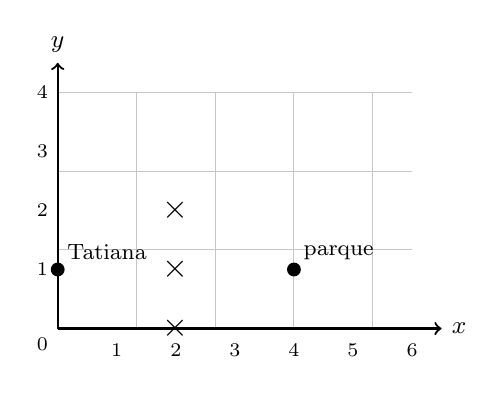
\begin{tikzpicture}[x=0.75cm, y=0.75cm, font=\footnotesize]
  \ejes{6}{4}
  \foreach \py in {0,1,2} \node[font=\large] at (2,\py) {$\times$};
  \fill (0,1) circle (2.5pt) node[above right] {Tatiana};
  \fill (4,1) circle (2.5pt) node[above right] {parque};
\end{tikzpicture}
\end{center}
\renglones{3}
\end{preguntas}

\begin{resumen}
\begin{itemize}
  \item Una trayectoria es el camino de un lugar a otro; se describe con instrucciones o con
        la lista de puntos por donde pasa.
  \item Su longitud es el número de cuadras recorridas.
  \item Hay varios caminos más cortos: todos tienen las mismas cuadras horizontales y
        verticales, en distinto orden.
  \item Un camino que da vueltas de más, o que rodea un obstáculo, es más largo.
\end{itemize}
\end{resumen}

\tema{Mapas y planos}\label{tema:mapas}

\begin{hilo}
Llegó el momento del mensaje final. Tatiana tiene una tarde libre y quiere conocer el barrio.
Con un mapa, un sistema de referencia y trayectorias bien escritas, puede recorrerlo sola.
\end{hilo}

Un \textbf{mapa} o \textbf{plano} representa un lugar visto desde arriba. El de este tema es un
\textbf{mapa simplificado}: las calles forman una cuadrícula, los números crecen hacia la
derecha (oriente) y hacia arriba (norte), como en el plano cartesiano, y cada lugar está en una
esquina. No es un mapa real de Cali ni está a escala: solo sirve para practicar coordenadas y
recorridos, contando cuadras.

\begin{center}
\begin{minipage}{\linewidth}
\centering
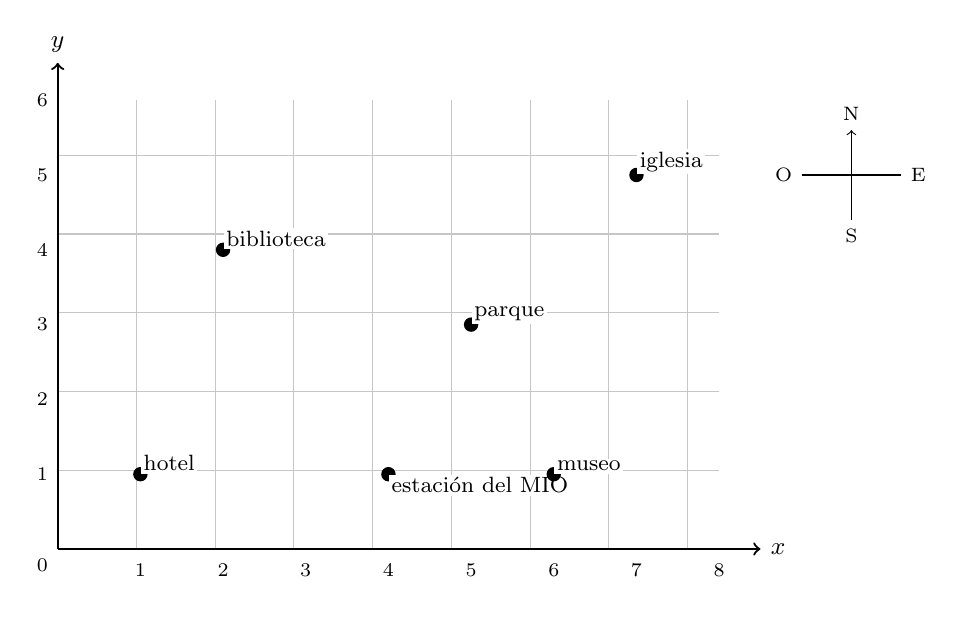
\begin{tikzpicture}[x=1.05cm, y=0.95cm, font=\footnotesize]
  \ejes{8}{6}
  \foreach \t/\px/\py/\pos in {hotel/1/1/above right, estación del MIO/4/1/below right,
      biblioteca/2/4/above right, parque/5/3/above right, iglesia/7/5/above right,
      museo/6/1/above right}
    {\fill (\px,\py) circle (2.6pt); \node[\pos, fill=white, inner sep=1pt] at (\px,\py) {\t};}
  \rosa{9.6,5}
\end{tikzpicture}

\vspace{1mm}
{\footnotesize Mapa simplificado del barrio (sin escala). Cada punto marca un lugar; cada lado
de un cuadro es una cuadra.}
\end{minipage}
\end{center}

% Ejercicio: ubicacion-5-017
\begin{ejemplo}[Del hotel al parque]
El parque está en $(5, 3)$. El hotel está en $(1, 1)$, así que desde el hotel hay que caminar
$5 - 1 = 4$ cuadras al oriente y $3 - 1 = 2$ cuadras al norte: 6 cuadras por un camino más
corto.
\end{ejemplo}

\Needspace{7\baselineskip}
\begin{aplicacion}[Los mapas oficiales de Colombia]
El Instituto Geográfico Agustín Codazzi publica en internet los mapas oficiales del país. Allí
cada municipio, río o carretera tiene coordenadas, y así una ambulancia, un avión o un equipo
de rescate llegan exactamente al lugar indicado~\cite{igac}.
\end{aplicacion}

\begin{preguntas}
% Ejercicio: ubicacion-5-018
\pregunta En el mapa del barrio, ¿qué lugar está en $(2, 4)$? ¿Y en $(6, 1)$? Escribe las
coordenadas de la iglesia y de la estación del MIO.
\renglones{2}
% Ejercicio: ubicacion-5-019
\pregunta Usa el mapa del barrio y los puntos cardinales. Describe dónde queda:
\begin{opciones}
  \item la iglesia respecto al parque;
  \item la biblioteca respecto al museo;
  \item el hotel respecto a la estación del MIO.
\end{opciones}
\renglones{3}
% Ejercicio: ubicacion-5-020
\pregunta \textbf{El mensaje para Tatiana.} Escríbele un mensaje con el recorrido hotel →
biblioteca → parque → iglesia: las coordenadas de cada lugar, las instrucciones de cada tramo
con puntos cardinales (por el camino más corto) y el total de cuadras.
\renglones{6}
% Ejercicio: ubicacion-5-021
\pregunta Tatiana propone otro orden: hotel → parque → biblioteca → iglesia. ¿Cuántas cuadras
camina así? ¿Cuál de los dos recorridos le conviene más y por qué?
\renglones{4}
\end{preguntas}

\begin{resumen}
\begin{itemize}
  \item Un mapa representa un lugar visto desde arriba; en un mapa simplificado en cuadrícula,
        cada lugar tiene coordenadas $(x, y)$.
  \item Con el norte arriba, la posición de un lugar respecto a otro se describe con puntos
        cardinales: cuántas cuadras al oriente u occidente y cuántas al norte o sur.
  \item Un buen recorrido da las coordenadas, las instrucciones de cada tramo y la longitud.
  \item El orden en que se visitan los lugares cambia la longitud total del recorrido.
\end{itemize}
\end{resumen}

% ---------------------------------------------------------------------
% 5. Cierre del hilo conductor
% ---------------------------------------------------------------------
\seccion{Cierre: dos números y un acuerdo}

Tatiana llegó a Cali sin conocer nada y ahora puede recorrer el barrio sola. No necesitó que
nadie la acompañara: le bastó un sistema de referencia, unos pares ordenados y trayectorias
escritas con claridad. Cualquier persona que lea su mensaje llega al mismo lugar. Es la misma
idea que tuvo Descartes hace casi cuatrocientos años y la que usó Katherine Johnson para que un
astronauta diera la vuelta a la Tierra y regresara.

En el próximo trimestre daremos un paso más: ya no solo ubicaremos puntos, sino que mediremos
las figuras que se forman con ellos, su perímetro y su área.

% ---------------------------------------------------------------------
% 6. Evaluación
% ---------------------------------------------------------------------
\matrizevaluacion
  {Reconoce los elementos de un sistema de referencia (ejes, origen, cuadrantes, coordenadas) y
   los puntos cardinales, y explica por qué importa el orden del par.}
  {Ubica y lee puntos del primer cuadrante, traduce entre instrucciones cardinales y pares
   ordenados, y describe, dibuja y compara trayectorias en un mapa.}
  {Escribe instrucciones claras y completas, pensando en quien las va a leer.}
  {Acuerda reglas comunes con sus compañeros y las respeta, porque sin un acuerdo el sistema de
   referencia no funciona.}

\autoevaluacion

\seguimientodocente

% ---------------------------------------------------------------------
% 7. Referencias
% ---------------------------------------------------------------------
\begin{referencias}
% verificado: https://mathshistory.st-andrews.ac.uk/Extras/Descartes_La_Geometrie/ — MacTutor: «La Géométrie… published as an appendix to Discours de la méthode (1637)»
\bibitem{descartes1637} Descartes, R. (1637). \emph{La géométrie}. Apéndice del \emph{Discours
  de la méthode}.
% verificado: https://plato.stanford.edu/cgi-bin/encyclopedia/archinfo.cgi?entry=descartes-mathematics — autora Mary Domski; Summer 2025 Edition, eds. E. N. Zalta y U. Nodelman; la entrada dice que AB y BC se toman como «oblique coordinates»
\bibitem{sepdescartes} Domski, M. (2025). Descartes' Mathematics. En E. N. Zalta y
  U. Nodelman (eds.), \emph{The Stanford Encyclopedia of Philosophy} (edición de verano de
  2025). https://plato.stanford.edu/entries/descartes-mathematics/
% verificado: https://handbook.fide.com/chapter/E012023 — FIDE Laws of Chess vigentes desde el 1 ene. 2023, Apéndice C: columnas a–h y filas 1–8; «e4»
\bibitem{fide} FIDE (2023). \emph{Laws of Chess}, Apéndice C: notación algebraica. Federación
  Internacional de Ajedrez.
% verificado: https://it.wikisource.org/wiki/Il_Saggiatore_(Favaro)/6 — Il Saggiatore, cap. 6 (ed. Favaro): pasaje del «grandissimo libro… scritto in lingua matematica»
\bibitem{galileo1623} Galilei, G. (1623). \emph{Il Saggiatore}. Roma: Giacomo Mascardi.
% verificado: https://geoportal.igac.gov.co/ — geoportal oficial del IGAC: visores de cartografía básica y mapas nacionales, departamentales y temáticos
\bibitem{igac} Instituto Geográfico Agustín Codazzi. \emph{Geoportal}. Consultado el 14 de
  septiembre de 2026. https://geoportal.igac.gov.co/
% verificado: https://wild.maths.org/ren%C3%A9-descartes-and-fly-ceiling — Millennium Mathematics Project, Universidad de Cambridge: «Legend has it that Descartes… was watching a fly on the ceiling»
\bibitem{nrichmosca} Millennium Mathematics Project, Universidad de Cambridge. René Descartes
  and the fly on the ceiling. \emph{Wild Maths}. Consultado el 14 de septiembre de 2026.
% verificado: https://gblumen.mineducacion.gov.co/cgi-bin/koha/opac-detail.pl?biblionumber=4785 — MEN 2016, Panamericana Formas e Impresos, ISBN 978-958-691-913-5
\bibitem{mendba} Ministerio de Educación Nacional (2016). \emph{Derechos Básicos de
  Aprendizaje V.2: Matemáticas}. Bogotá: MEN.
% verificado: https://www.nasa.gov/centers-and-facilities/langley/katherine-johnson-biography/ — trayectoria de Freedom 7 (Shepard, mayo de 1961); Glenn: «If she says they're good, then I'm ready to go» (1962)
\bibitem{nasajohnson} NASA. \emph{Katherine Johnson biography}. Langley Research Center.
  Consultado el 14 de septiembre de 2026.
\end{referencias}

\end{document}
